\subsection{UC4 - Inserimento ATTIVITÀ\textsubscript{G} in EMT\textsubscript{G}}
\begin{itemize}
    \item \textbf{Identificativo}: UC4 
    \item \textbf{Nome}: Inserimento ATTIVITÀ\textsubscript{G} in EMT\textsubscript{G}
    \item \textbf{Descrione grafica}:
\end{itemize}
\begin{center}
    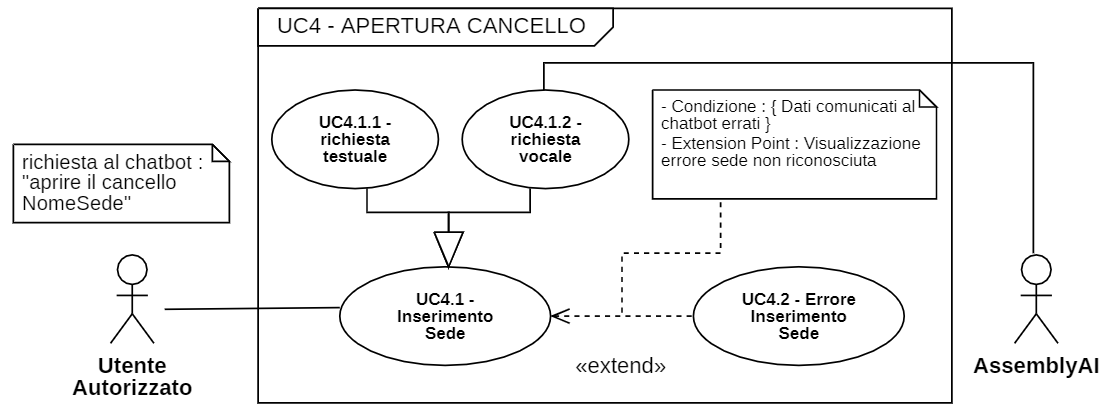
\includegraphics[scale=0.40]{images/UC4.png} 
\end{center}
\begin{itemize}
    \item \textbf{Attori}
    \begin{itemize} 
        \item \textit{Primari}: utente autorizzato
        \item \textit{Secondari}: non presenti
    \end{itemize}
 \item \textbf{Precondizione}: l'utente si è autenticato con sucesso, si trova nella schemata in cui comunica con il chabot con l'intenzione di registrare un'attività svolta. 
 \item \textbf{Postcondizione}: l'utente è riuscito con successo ad inserire la propria attività nel sistema EMT\textsubscript{G}.  
 \item \textbf{Scenario principale}: L'utente comunica al chatbot di voler consultivare un'attività. Il chatbot porrà dei quesiti all'utente al fine di ottenere le seguenti informazioni: 
    \begin{itemize}
        \item L'attività che si vuole consultivare (UC4.1)
        \item Numero di ore che sono state necessarie per svolgere l'attività (UC4.2)
        \item Il progetto a cui l'attività fa riferimento (UC4.3)
        \item Il luogo dove è stata svolta l'attività (UC4.4)
    \end{itemize}
 Durante tale processo è possibile che si verifichino degli errori, tra cui: 
    \begin{itemize}
        \item Il chatbot non è stato in grado di interpretare un messaggio fornito dall'utente (UC2)
        \item Il chatbot comunica che si è verificato un errore che non ha permesso di completare l'operazione richiesta, invitando l'utente a riprovare. (UC10)
        \item Il chatbot segnala un errore sul progetto indicato dall'utente nel caso in cui non esista. (UC20)
        \item Il chatbot segnala un errore sulla sede indicata dall'utente nel caso in cui non esista. (UC19)
    \end{itemize}
\end{itemize}

\newpage

\subsubsection{UC4.1 - Inserimento tipo di ATTIVITÀ\textsubscript{G}}

\begin{itemize}
    \item \textbf{Identificativo}: UC4.1 
    \item \textbf{Nome}: Inserimento tipo ATTIVITÀ\textsubscript{G} 
    \item \textbf{Descrione grafica}: (approfondita in UC4)
    \item \textbf{Attori}
        \begin{itemize} 
            \item \textit{Primari}: utente autorizzato
            \item \textit{Secondari}: non presenti
        \end{itemize}
    \item \textbf{Precondizione}: l'utente ha espresso la volontà di registrare un'attività. 
    \item \textbf{Postcondizione}: l'utente ha comunicato al chatbot il tipo di attività che vuole registrare. 
    \item \textbf{Scenario principale}: L'utente comunica al chatbot il tipo di attività da consultivare in maniera testuale (UC4.1.1) oppure vocale (UC4.1.2). L'operazione può andare a buon fine o può essere visualizzato un messaggio di errore nel caso in cui il tipo di attività non sia valido (UC4.5).
\end{itemize}

\subsubsection{UC4.2 - Inserimento ore da consultivare}
\begin{itemize}
    \item \textbf{Identificativo}: UC4.2 
    \item \textbf{Nome}: Inserimento ore da consultivare  
    \item \textbf{Descrione grafica}: (approfondita in UC4)
    \item \textbf{Attori}
        \begin{itemize} 
            \item \textit{Primari}: utente autorizzato
            \item \textit{Secondari}: non presenti
        \end{itemize}
    \item \textbf{Precondizione}: l'utente sta comunicando con il chatbot per inserire un'attività a consultivo. 
    \item \textbf{Postcondizione}: l'utente ha comunicato le ore da consultivare. 
    \item \textbf{Scenario principale}: all'interno dello scenario di registrazione di un'attività il chatbot chiede all'utente di inserire le ore che hanno coinvolto lo svolgimento. L'utente procede con l'inserimento dell'informazione in maniera testuale o vocale. L'operazione può andare a buon fine o può essere visualizzato un messaggio di errore nel caso in cui le ore inserite non siano valide (UC4.6).
\end{itemize}
\newpage

\subsubsection{UC4.3 - Inserimento progetto da consultivare}
\begin{itemize}
    \item \textbf{Identificativo}: UC4.3 
    \item \textbf{Nome}: Inserimento progetto da consultivare  
    \item \textbf{Descrione grafica}: (approfondita in UC4)
    \item \textbf{Attori}
        \begin{itemize} 
            \item \textit{Primari}: utente autorizzato
            \item \textit{Secondari}: non presenti
        \end{itemize}
    \item \textbf{Precondizione}: l'utente sta comunicando con il chatbot per inserire un'attività a consultivo. 
    \item \textbf{Postcondizione}: l'utente ha fornito il progetto correlato all'attività svolta al chatbot. 
    \item \textbf{Scenario principale}: l'utente tramite un messagio testuale o vocale, comunica al chatbot il nome del progetto per l'attività che sta inserendo. Tale progetto, se valido, porterà alla continuazione dell'inserimento, altrimenti il chatbot visualizzerà un messaggio di errore (UC4.7). 
\end{itemize}

\subsubsection{UC4.4 - Inserimento luogo attività}
\begin{itemize}
    \item \textbf{Identificativo}: UC4.4
    \item \textbf{Nome}: Inserimento luogo  attività  
    \item \textbf{Descrione grafica}: (approfondita in UC4)
    \item \textbf{Attori}
        \begin{itemize} 
            \item \textit{Primari}: utente autorizzato
            \item \textit{Secondari}: non presenti
        \end{itemize}
    \item \textbf{Precondizione}: l'utente sta comunicando con il chatbot per inserire un'attività a consultivo. 
    \item \textbf{Postcondizione}: l'utente ha fornito al chatbot il luogo in cui ha svolto tale attività. 
    \item \textbf{Scenario principale}: l'utente tramite un messagio testuale o vocale, comunica al chatbot il luogo dove è stata svolta l'attività che sta inserendo. Tale luogo, se valido, porterà alla continuazione dell'inserimento, altrimenti il chatbot visualizzerà un messaggio di errore (UC4.8). 
\end{itemize}

\subsubsection{UC4.5 - Errore inserimento ATTIVITÀ\textsubscript{G}}
\begin{itemize}
    \item \textbf{Identificativo}: UC4.5
    \item \textbf{Nome}: Errore inserimento ATTIVITÀ\textsubscript{G}
    \item \textbf{Descrione grafica}: (approfondita in UC4)
    \item \textbf{Attori}
        \begin{itemize} 
            \item \textit{Primari}: utente autorizzato
            \item \textit{Secondari}: non presenti
        \end{itemize}
    \item \textbf{Precondizione}: l'utente ha fornito il nome dell'attività in un formato non valido. 
    \item \textbf{Postcondizione}: chatbot comunica all'utente la non validità dell'attività fornita.
    \item \textbf{Scenario principale}: l'utente fornisce il nome di un'attività da consultivare che non risulta essere valido. Il chatbot notifica l'errore e chiede all'utente di riprovare l'inserimento. 
\end{itemize}

\subsubsection{UC4.6 - Errore inserimento ore}
\begin{itemize}
    \item \textbf{Identificativo}: UC4.6
    \item \textbf{Nome}: Errore inserimento ore
    \item \textbf{Descrione grafica}: (approfondita in UC4)
    \item \textbf{Attori}
        \begin{itemize} 
            \item \textit{Primari}: utente autorizzato
            \item \textit{Secondari}: non presenti
        \end{itemize}
    \item \textbf{Precondizione}: l'utente ha fornito un numero di ore relativo all'attività in un formato non valido. 
    \item \textbf{Postcondizione}: chatbot comunica all'utente la non validità delle ore fornite.
    \item \textbf{Scenario principale}: l'utente fornisce il numero di ore di un'attività da consultivare che non risulta essere valido. Il chatbot notifica l'errore e chiede all'utente di riprovare l'inserimento. 
\end{itemize}
\newpage

\subsubsection{UC4.7 - Errore inserimento progetto}
\begin{itemize}
    \item \textbf{Identificativo}: UC4.7
    \item \textbf{Nome}: Errore inserimento progetto
    \item \textbf{Descrione grafica}: (approfondita in UC4)
    \item \textbf{Attori}
        \begin{itemize} 
            \item \textit{Primari}: utente autorizzato
            \item \textit{Secondari}: non presenti
        \end{itemize}
    \item \textbf{Precondizione}: l'utente ha fornito un nome di progetto relativo all'attività in un formato non valido. 
    \item \textbf{Postcondizione}: chatbot comunica all'utente la non validità del nome del progetto fornito.
    \item \textbf{Scenario principale}: l'utente fornisce il nome del progetto di un'attività da consultivare che non risulta essere valido. Il chatbot notifica l'errore e chiede all'utente di riprovare l'inserimento. 
\end{itemize}

\subsubsection{UC4.8 - Errore inserimento luogo}
\begin{itemize}
    \item \textbf{Identificativo}: UC4.8
    \item \textbf{Nome}: Errore inserimento luogo
    \item \textbf{Descrione grafica}: (approfondita in UC4)
    \item \textbf{Attori}
        \begin{itemize} 
            \item \textit{Primari}: utente autorizzato
            \item \textit{Secondari}: non presenti
        \end{itemize}
    \item \textbf{Precondizione}: l'utente ha fornito un luogo relativo all'attività in un formato non valido. 
    \item \textbf{Postcondizione}: chatbot comunica all'utente la non del luogo fornito.
    \item \textbf{Scenario principale}: l'utente fornisce il luogo dove ha svolto un'attività da consultivare, non risultando essere valido. Il chatbot notifica l'errore e chiede all'utente di riprovare l'inserimento. 
\end{itemize}
\newpage